\chapter{Graph}

Graph merupakan sebuah \textit{Abstract Data Type} (ADT) yang digunakan untuk mengimplementasikan konsep \textit{graph} dan \textit{directed graph} dalam matematika. Dalam matematika sendiri, graph merupakan sebuah representasi dari sekumpulan objek yang saling terhubung. Objek-objek yang ada di dalam graph dikenal dengan nama \textit{vertex}, sedangkan hubungan (penghubung) antar objek tersebut dikenal dengan nama \textit{edge}.

Sebuah graph dapat digunakan untuk merepresentasikan banyak hal dalam dunia nyata. Misalnya, kita dapat merepresentasikan pohon pengetahuan dalam sebuah graph seperti yang nampak pada gambar~\ref{fig:knowledge-tree}. Peta juga kerap kali direpresentasikan sebagai graph, dengan titik-titik pergerakan sebagai vertex-nya, dan jalur antar titik sebagai edge-nya (lihat gambar~\ref{fig:map-graph}).

\begin{figure}
    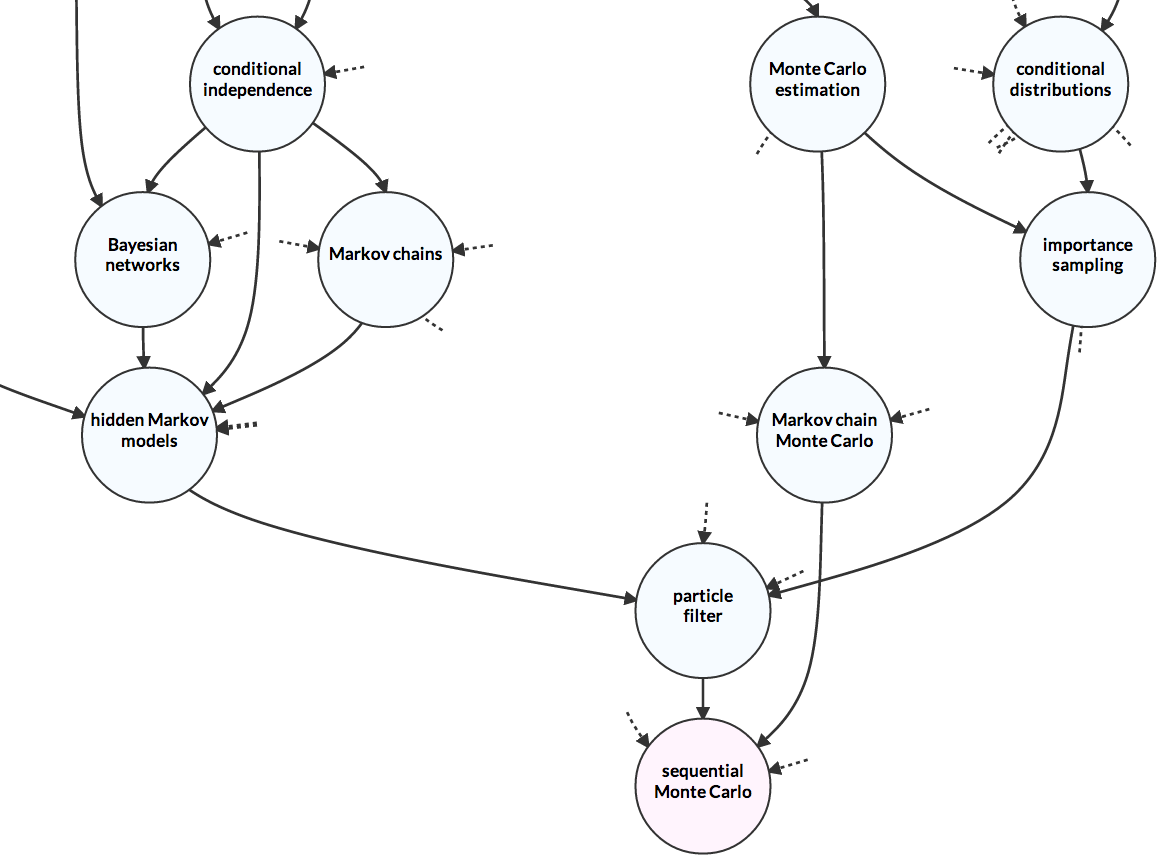
\includegraphics[width=\textwidth,keepaspectratio]{fig/KnowledgeTree.png}%
	\caption{Pohon Pengetahuan}%
	\label{fig:knowledge-tree}%
\end{figure}

\begin{figure}
    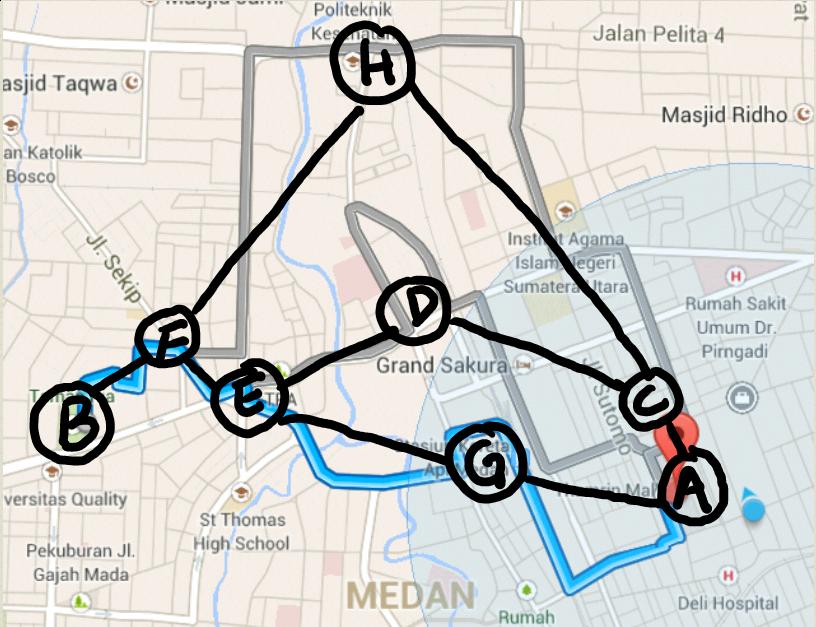
\includegraphics[width=\textwidth,keepaspectratio]{fig/DirectedGraphMap.png}%
	\caption{Peta dengan Graph}%
	\label{fig:map-graph}%
\end{figure}

Terdapat sangat banyak jenis dan definisi dari graph, yang masing-masing memiliki kegunaan spesifik dan kelebihan serta kekurangan tersendiri. Pada bagian ini kita hanya akan membahas satu jenis graph, yaitu graph tidak berarah yang berlabel. Untuk mengetahui lebih lanjut mengenai detil dari berbagai jenis graph serta kelebihan dan kekurangannya, silahkan baca buku atau modul tentang struktur data terkait.

Graph tidak berarah berlabel yang kita gunakan didefinisikan sebagai berikut:

\begin{itemize}
    \item Sebuah graph didefinisikan sebagai $G = (V, E)$.
    \item $V$ merupakan sekumpulan vertex.
    \item $E$ merupakan sekumpulan edge.
    \item $E = (V1, V2, v)$ di mana $V1$ dan $V2$ adalah dua buah vertex yang terhubung dan $v$ adalah label (bobot; jarak) dari kedua vertex tersebut.
    \item Dua buah vertex yang saling berdampingan membentuk sebuah edge dapat dihubungkand engan simbol $~$, sehingga $u ~ v$ dapat dibaca sebagai vertex $u$ dan $v$ yang berdampingan (memiliki edge).
\end{itemize}

Definisi graph yang kita gunakan tidak terlalu jauh berbeda dengan yang digunakan pada teori graph dalam matematika pada umumnya. Tetapi ingat bahwa definisi ini seringkali dimodifikasi sesuai dengan kebutuhan dan tujuan dari algoritma yang menggunakan graph tersebut. Misalnya, representasi dan definisi dari sebuah graph yang digunakan untuk menyelesaikan permasalahan pemetaan seperti mencari jalur terpendek akan berbeda dengan representasi untuk menyelesaikan masalah deteksi bahasa. Begitupun, algoritma-algoritma dasar yang sama dapat kita immplementasikan pada representasi graph yang berbeda ini (misalnya: algoritma untuk pencarian jalur terpendek). Perbedaan hanya akan ditemukan pada detil implementasi nantinya.

Untuk memperjelas pengertian tentang representasi graph yang berbeda, kita akan melihat beberapa jenis cara merepresentasikan graph yang umum digunakan.

\section{Representasi Graph}

Secara umum terdapat tiga metode untuk merepresentasikan graph dalam ilmu komputer, yaitu:

\begin{enumerate}
    \item Adjacency List
    \item Adjacency Matrix
    \item Incidence Matrix
\end{enumerate}

\subsection{Graph dengan Adjacency List}

\subsection{Graph dengan Adjacency Matrix}

\subsection{Graph dengan Incidence Matrix}

\section{Operasi Umum Graph}

Terdapat beberapa operasi umum yang dapat dilakukan terhadap graph, yaitu:

\begin{enumerate}
    \item Penambahan Vertex baru
    \item Penambahan Edge baru
    \item Penghapusan Vertex
    \item Penghapusan Edge
    \item Pengecekan apakah dua buah vertex terhubung
\end{enumerate}

Kompleksitas dari masing-masing operasi sendiri berbeda-beda, tergantung dari cara representasi graph yang kita gunakan

\section{Contoh Implementasi Graph}
